\section{Design of \tool}

\subsection{Definitions}\label{sec:toolDefs}
\noindent
{\bf System Entity.} In this work, we distinguish five principal entity categories: \textit{Processes}, \textit{Files}, \textit{Registry}, \textit{Dynamic Link Libraries (DLLs)}, and \textit{Network Connections}, the latter typically denoted by sockets. System entities possess unique attributes: the attributes associated with \textit{process} entities might include their Process ID (pid) or their executable paths. 

\noindent
{\bf System Event.} In this work, a system event $e$ is given by a tuple $\langle src, dst, rel, time\rangle$, where $src$ designates the source entity, constrained to only process entities, $dst$ indicates the target or destination entity, $rel$ denotes their interaction nature (e.g., writing into a file), and $time$ specifies the timestamp of the event occurrence.
We also illustrated the temporal relationship between events as $\langle e_1 \to e_2 \to e_3 \rangle$, indicating that the events occur in a logical sequence. 

% \noindent
% {\bf Proposition Definition.}
% A proposition is represented as a triplet $\langle src, operation, dst\rangle$, where:
% \begin{itemize}
%     \item $src$ and $dst$ represent entities.
%     \item Entities can be: Process, Dll, Registry, File, IP:port.
%     \item An operation is performed from the $src$ to the $dst$.
% \end{itemize}

\noindent
{\bf Behavioral Invariant.} In this work, the behavioral invariant is defined as follows:
\begin{align*}
 & \mathcal{I}  ::= \ \phi \mid \phi \wedge \mathcal{I} \\
 & \phi  \ \ \in \ \{ P_{ep}(x,y), \ P_{pp}(x,Y), \ P_{cp}(x,Y), \ P_{a}(x,y), \ P_{o}(x_1,x_2,\ldots)\} \\
\end{align*}
where $P_{ep}(x,y)$ (resp. $P_{pp}(x,y)$) indicates that the execution path (parent process) of process $x$ is $y$, $P_{cp}(x, Y)$ indicates that the child processes of $x$ must come from processes set $Y$, $P_{a}(x,y)$ denotes that the process $x$ must execute the action $y$ in the future, and the $P_{o}(x_1,x_2,\ldots)$ requires that the processes must be executed in the sequential order of $x_1,x_2,\ldots$.

For example, a behavior invariant $\mathcal{I}_e$ of \texttt{svchost.exe} can be represented by the conjunction of the following set: 

\begin{center}
$ \left\{
\begin{array}{c}
P_{ep}(\texttt{svchost.exe}, \text{``C:/windows/system32/''}),\\
 P_{pp}(\texttt{svchost.exe}, \texttt{services.exe}),\\
 P_{a}(\texttt{svchost.exe}, \text{Load(\texttt{advapi32.dll})})
\end{array} \right\}$
\end{center}

which states that the execution path of \texttt{svchost.exe} should be \text{"C:/windows/system32/"}, with parent process 
as \texttt{services.exe}, and it will load \texttt{advapi32.dll} finally.


\subsection{Process Classification}
We created a prompt to query LLMs that classified these processes into legitimate, illegitimate, and uncertain names (due to the LLMs database's incompleteness).
Due to name confusion, many illegitimate process names can be changed to legitimate process names for further evaluation.
For both the legitimate and confusion processes, we construct profiles according to the methods described in the following sections. An investigator should investigate further illegitimate or unclear categories since they may contain malware.


\subsection{Behavioral Reference Construction}
In this section, we describe the methodology for constructing Behavioral References for processes, which can be categorized into three phases. 
This method combines the strengths of Language Model (LLM) agents, particularly utilizing Retrieval Augmented Generation (RAG) and Direct Query LLMs, to create accurate and diverse command sets, sandbox testing environments for empirical validation, and algorithmic extraction of behavioral invariants based on common and frequent item mining. The framework aims to mitigate the phenomenon of "hallucinations" in LLM outputs through a multifaceted validation strategy.


\subsubsection{Retrieval Augmented Generation (RAG)}
To generate accurate command sets, we first implement the Retrieval Augmented Generation (RAG) method, and second, to generate a more diverse, we utilize Direct Querying of LLMs for the generation of process behavior trees. Together, these two steps collaborate to produce accurate and diversified commands.

\noindent
{\bf Utilizing Search Engines}: Initially, the RAG system employs a search engine, such as Google, to perform a broad and comprehensive search based on the user's query. This step is about casting a wide net to ensure no relevant document is overlooked.

\noindent
{\bf Retrieving Top Documents}: From the search results, the system selects the top $N$ documents. The selection criteria hinge on relevance to the query, recency, and the credibility of the sources. These documents are pre-indexed in a database that the RAG system can query.

\noindent
{\bf Indexing for Quick Access}: Each document is broken down into manageable chunks or vectors, with key concepts and information encoded into embeddings. These embeddings act as a map to the knowledge landscape within each document, allowing for rapid and efficient retrieval of information.

\noindent
{\bf Indexing and Retrieval}: The RAG system begins by searching through a pre-indexed database of documents to find chunks of text relevant to the user's query based on the prompt as shown in Appendix~\ref{prompt-rag-commands}. This is analogous to sourcing current and contextual data that can inform the behavior of the process.

\noindent
{\bf Command Generation through Contextual Relevance}: The system then retrieves documents that appear to have the highest relevance to the process in question. For instance, in a process related to data privacy, RAG might retrieve the latest legal regulations, industry best practices, and recent case studies.


\subsubsection{Process Behavior Tree Construction}
The construction of \textit{Process Behavior Trees} is one of the most important steps in the process.
First, we define the \textit{Process Behavior Tree}.
\begin{figure}[h]
    \centering
      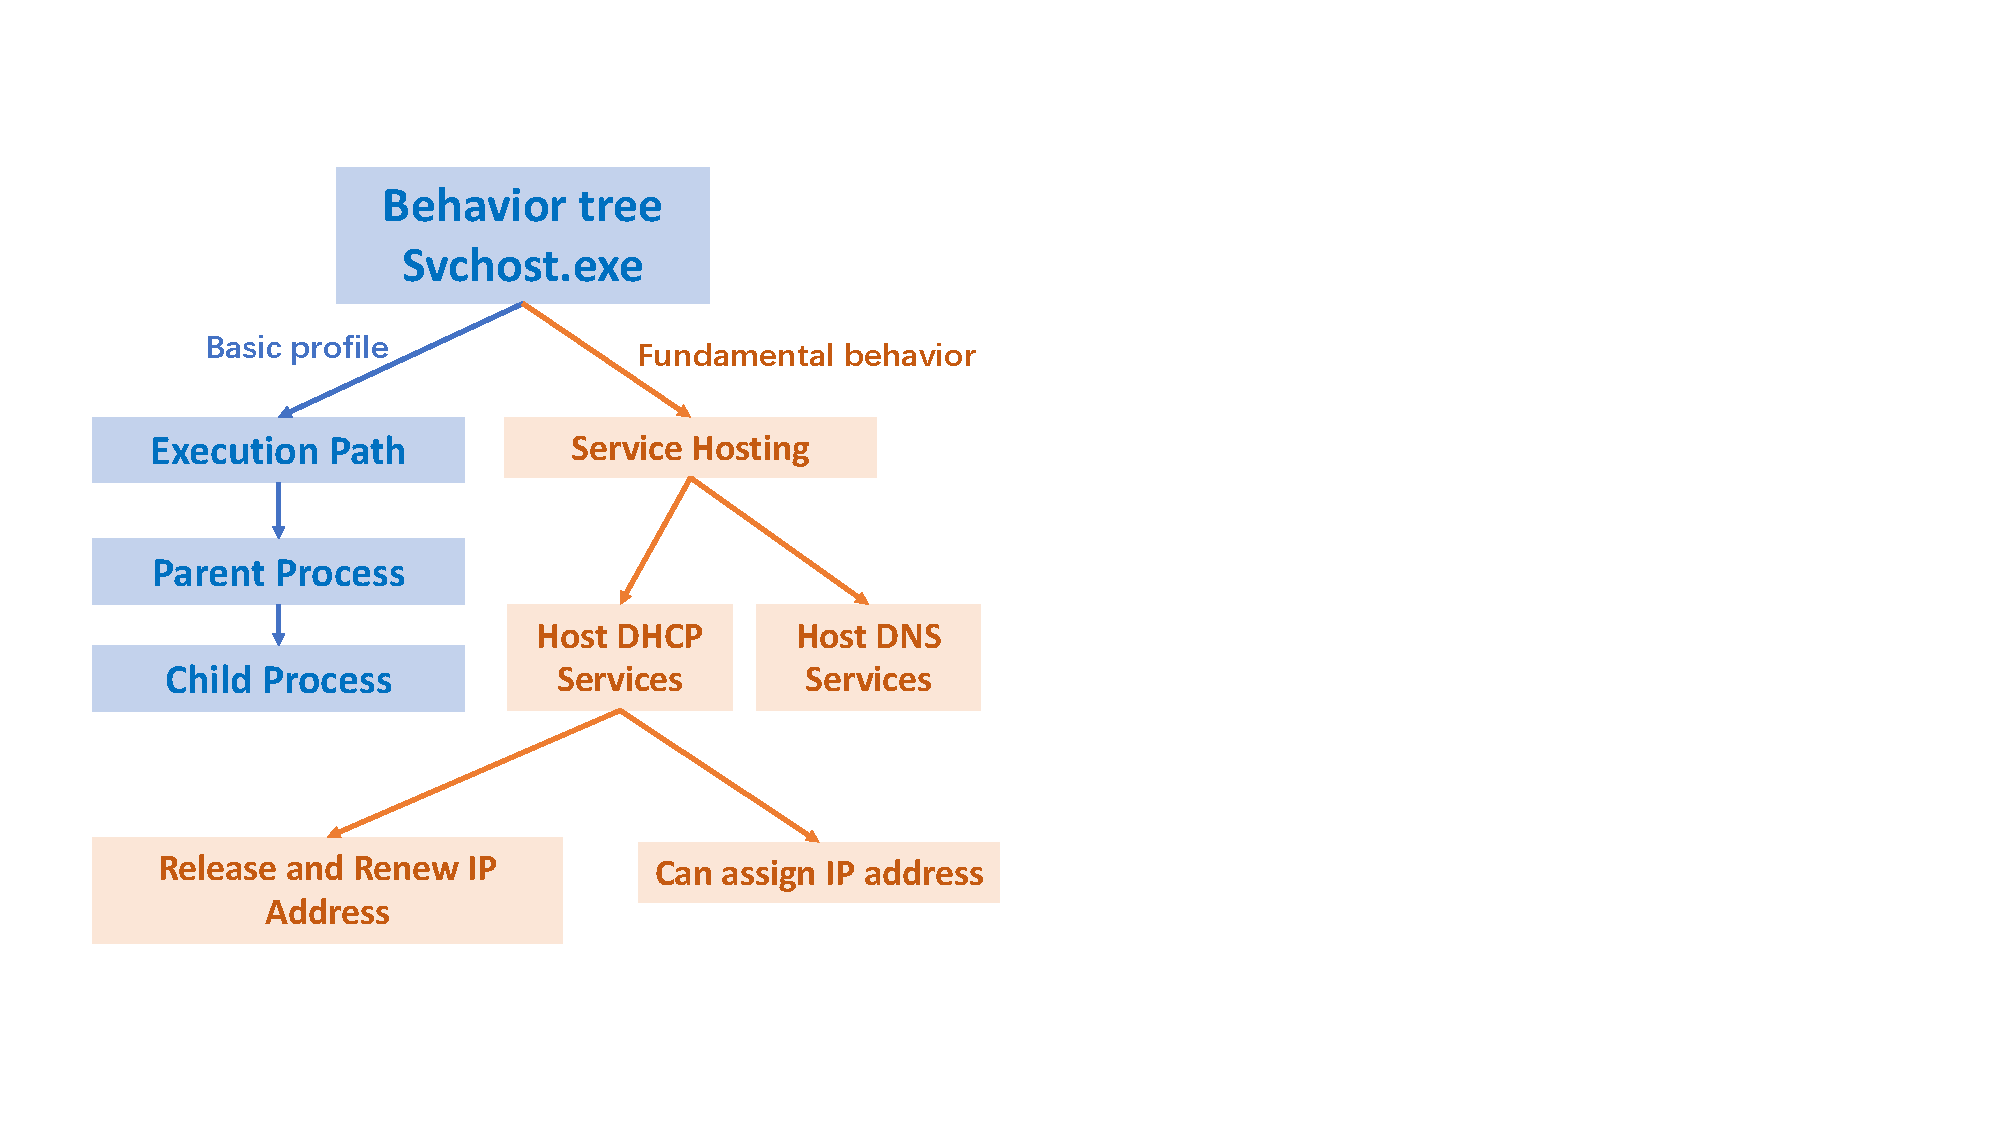
\includegraphics[width=0.35\textwidth]{figs/tree1.pdf}
    \caption{Process Behavior Tree Representation.}
    \label{fig:BT}
\end{figure}

To generate as many behaviors as possible, we've crafted two prompts: the \textit{Initialization Behavior Tree Prompt}(A detailed prompt can be found in the Appendix~\ref{prompt-init-tree}) and the \textit{Expansion Behavior Tree Prompt}. Initially, we employ the \textit{Initialization Behavior Tree Prompt} to create a foundational behavior tree. Subsequently, this tree is expanded through iterative rounds using the \textit{Expansion Behavior Tree Prompt}.

The resulting behavior tree is illustrated in Figure~\ref{fig:BT}. Taking the behavior tree of \textit{svchost.exe} as an example, we begin with the basic profile. This includes details such as the execution path of the process, its parent process (the parent process of \textit{svchost.exe} can only be \textit{services.exe}), and its child processes. Following this, we have the fundamental behaviors, such as service hosting, DLL loading, and service isolation exhibited by \textit{svchost.exe}. Focusing on the most significant behavior, which is service hosting, the behavior tree can be extended to detail the specific services being hosted. 

\subsubsection{Feedback-based Command Execution}
Following command generation, the next step involves the creation of an automated sandbox testing environment. Within this environment, the generated commands are executed, and logs for each command's behavior are collected. These logs serve as the foundation for the subsequent extraction of behavioral invariants, facilitating a deeper understanding of the process's dynamics and ensuring the commands' validity.

The stage of command execution is a critical juncture in the process of Behavioral Reference Construction, where the practical viability of generated commands is put to the test. This phase involves a sophisticated feedback loop within an automated sandbox testing environment to refine and perfect the command set for assured success upon execution.

\noindent
{\bf Execution in Automated Sandbox}:
An automated sandbox environment is set up to provide an isolated testing ground for the execution of commands, simulating actual operational conditions while protecting the main system from potential negative impacts of untested commands. During this phase, commands generated earlier are input into the sandbox, where each command's execution is meticulously monitored, with the system recording its behavior, results, and any errors that occur.

\noindent
{\bf Error Feedback Mechanism}:
In the quest for precision, the execution phase includes an error feedback mechanism to address failures in command execution from the previous stage. Common errors identified involve incompatible parameter combinations, such as using -h for file or printer sharing with -k for registry keys, which targets incompatible objects. There are also instances of misformatted commands, like pairing -f, which displays full process token information, with -c for Windows services, leading to a context mismatch. Additionally, issues with erroneous or missing parameter values are frequent, such as a command where -f is used without an accompanying account list after -p for specifying a process name or PID. To rectify these issues, an error correction loop is formed, leveraging both the LLM and sandbox outputs to iteratively refine commands. This loop represents a dynamic interplay between the LLM's generative abilities and the empirical data from the sandbox, substantially improving the success rate of command executions.

\noindent
{\bf Knowledge Augmentation Feedback}:
To enhance command generation further, the system integrates feedback on the relationships between parameters, including conflicts and dependencies. Conflicts arise when certain parameters, like -h and -k or -p and -c, cannot coexist due to their differing object applications. Conversely, dependencies are noted where parameters should be used together, such as -l with -i for displaying security descriptors excluding inherited ACEs, or -f with -p for full process token information. Through this systematic refinement, the system strengthens its grasp on parameter conflicts and dependencies, significantly boosting the accuracy of command generation by ensuring that only compatible and contextually relevant parameters are paired.



\subsubsection{Behavioral Invariants Extraction}

The final phase of the framework focuses on extracting Behavioral Invariants using algorithms for mining common and frequent items. This step leverages both traditional algorithms and the interpretive capabilities of LLMs to identify invariant behaviors within processes, enhancing the robustness of the Behavioral Reference Construction.

\begin{figure*}[h]
  \begin{subfigure}{.45\textwidth}
      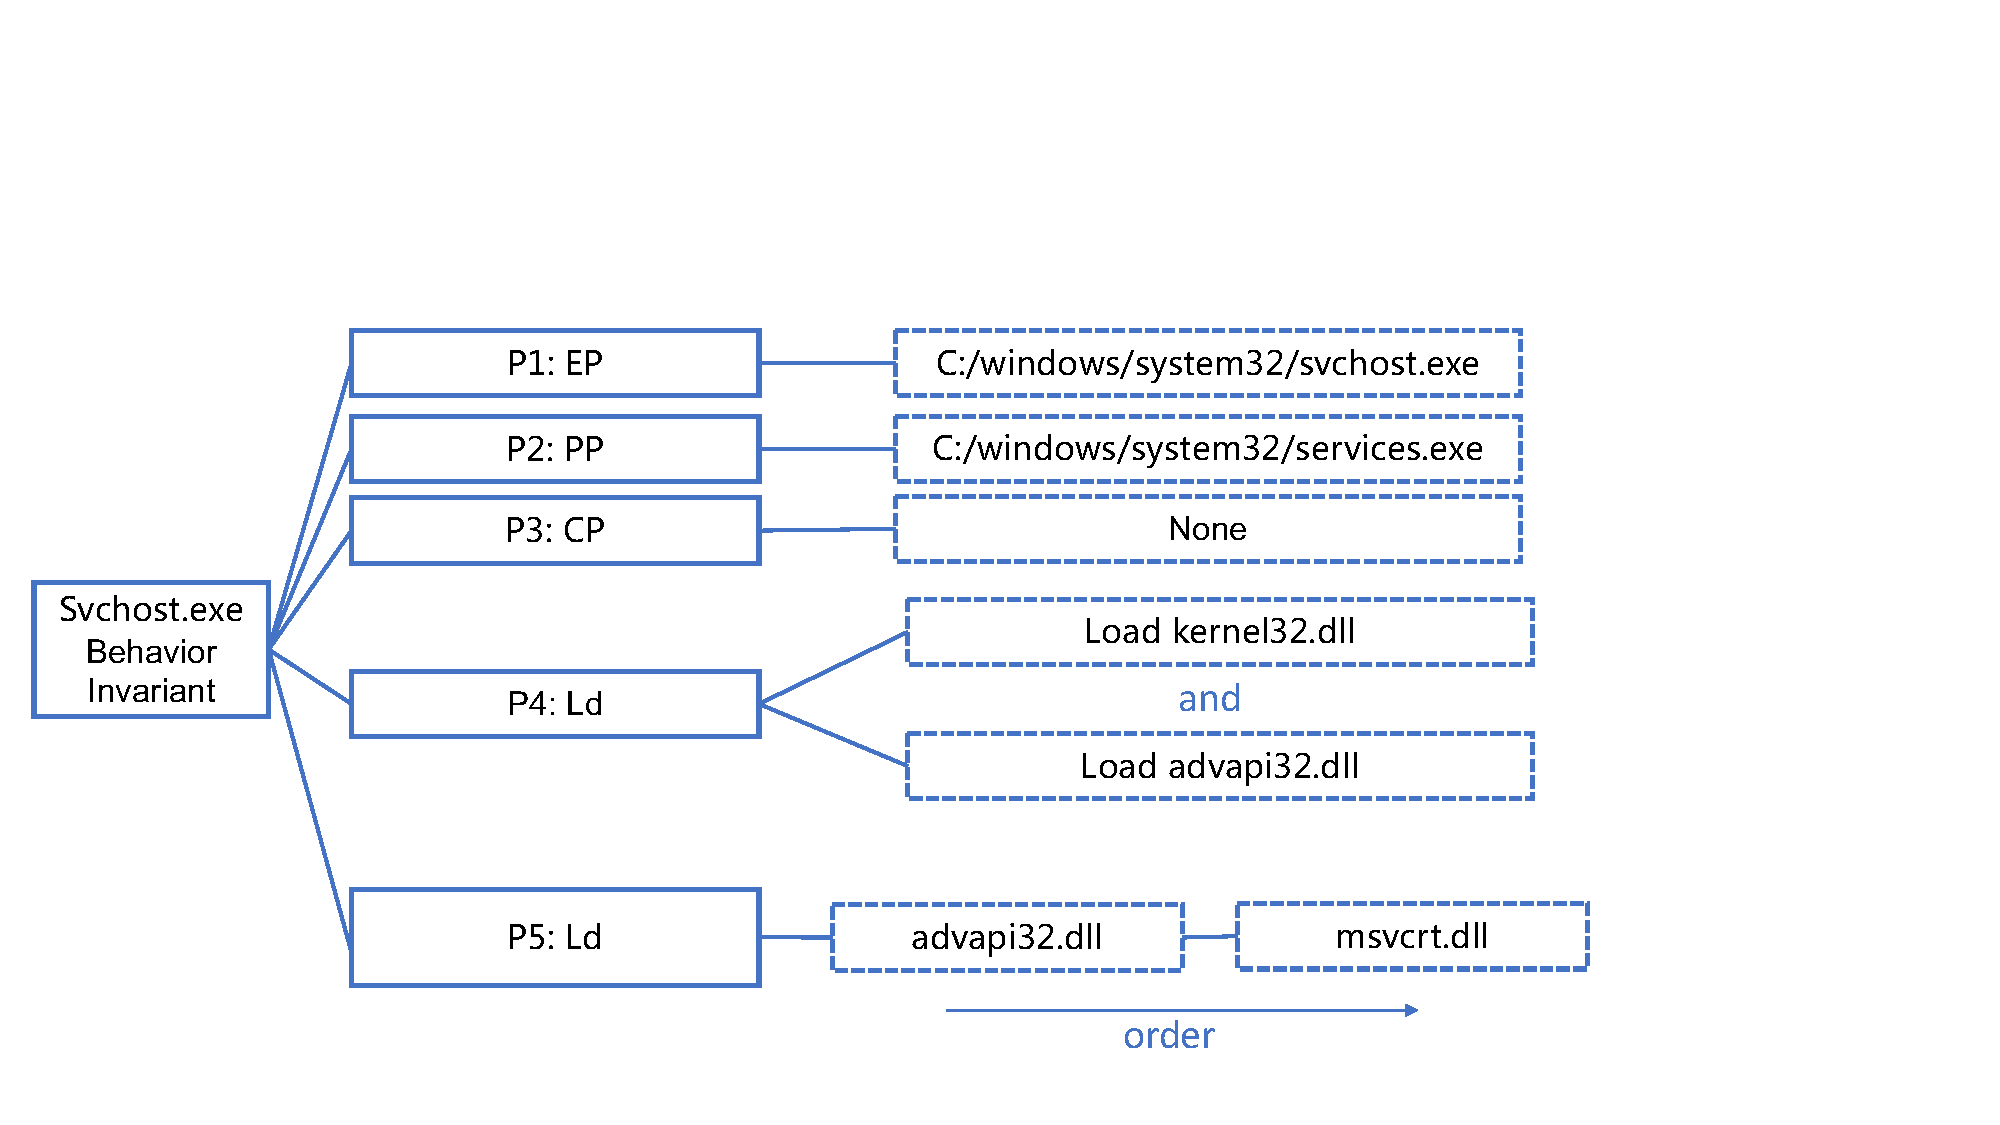
\includegraphics[width=\textwidth]{figs/cons-svchost.pdf}
      \caption{Behavioral Invariants of Svchost}
      \label{fig:cons-svchost}
  \end{subfigure}
  \hfill
  \begin{subfigure}{.5\textwidth}
      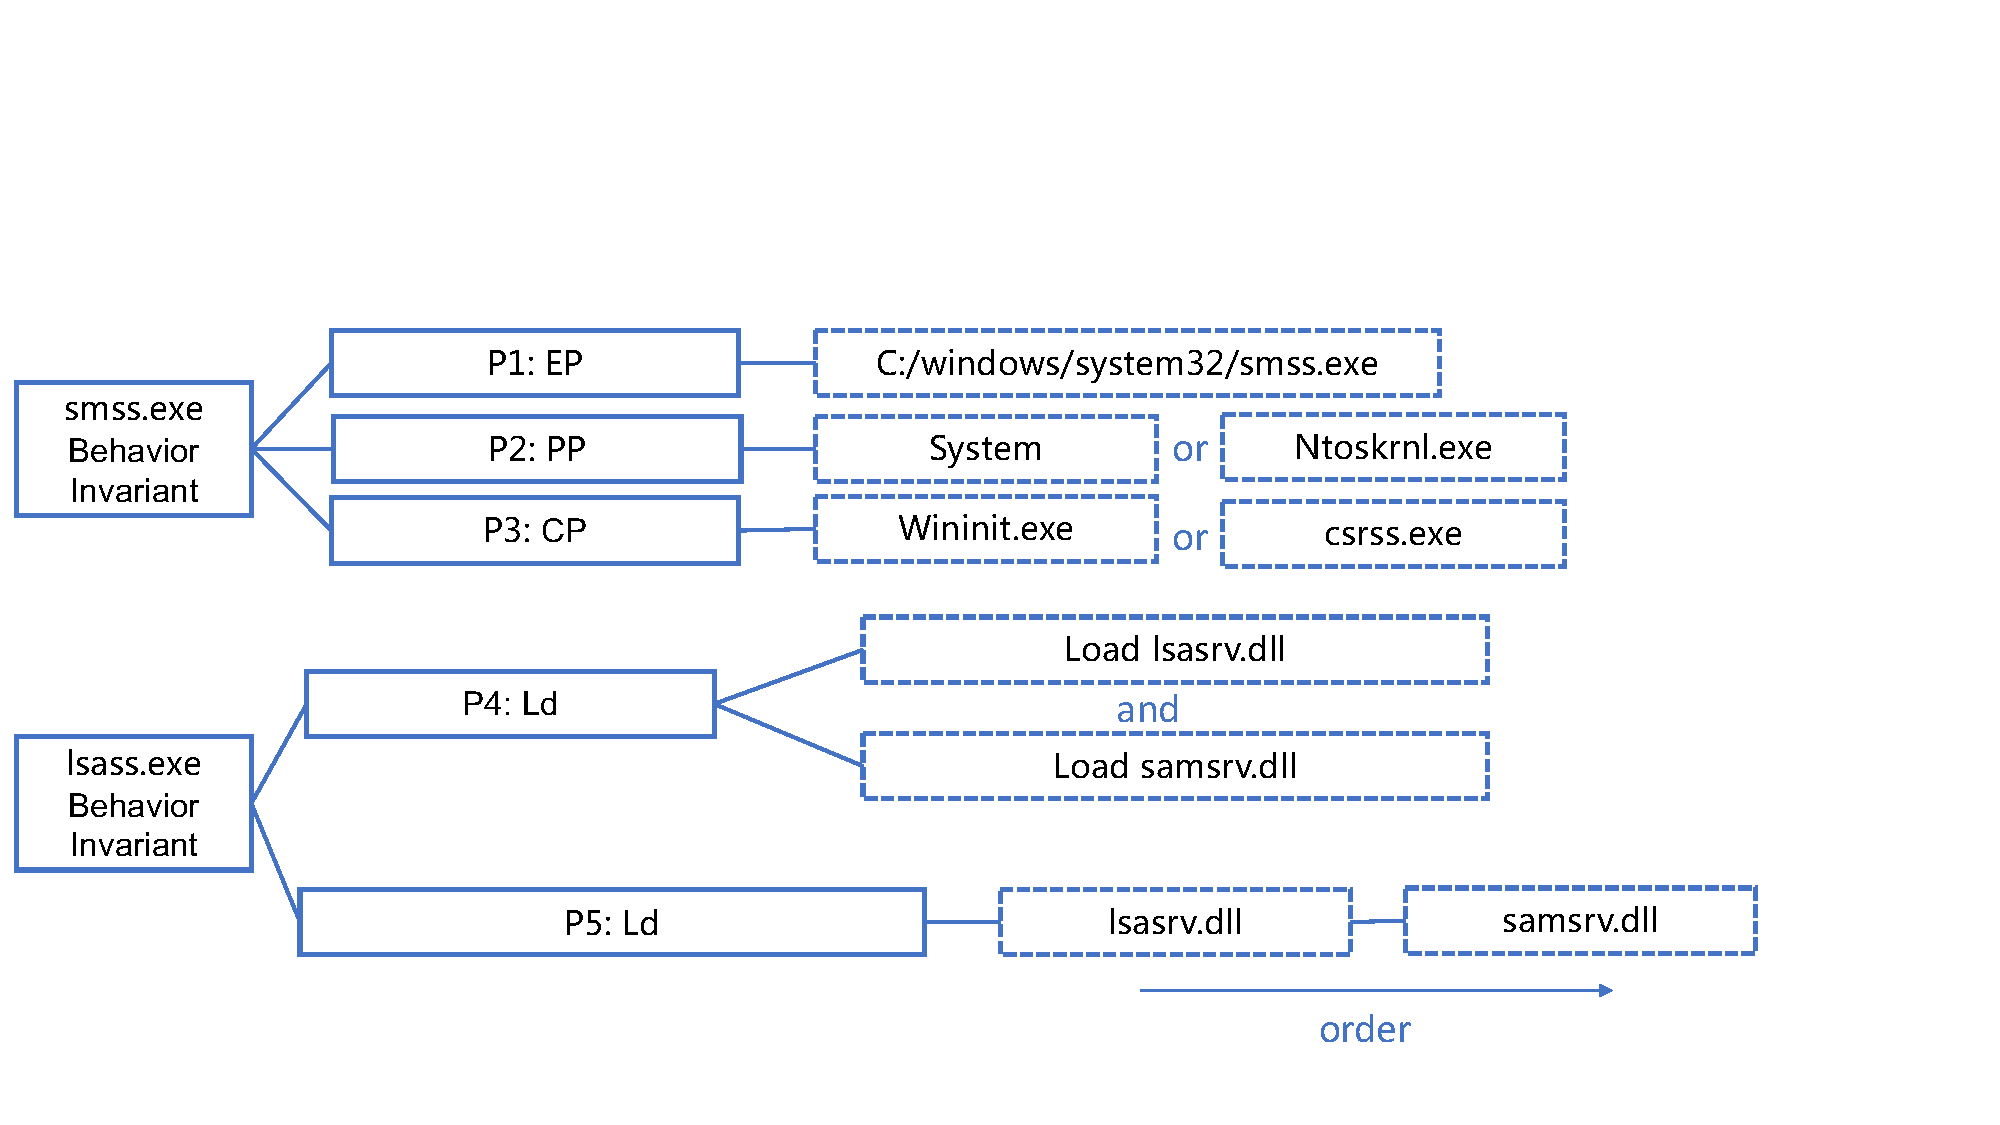
\includegraphics[width=\textwidth]{figs/cons-smss-lsass.pdf}
      \caption{Behavioral Invariants of Smss and Lsass}
      \label{fig:cons-smss-lsass}
  \end{subfigure}
  \hfill
  \caption{Behavioral Invariants: 'EP' stands for Execution Path, 'PP' represents Parent Process, 'CP' is for Child Process, and 'LD' refers to Load.}
  \label{fig:cons-def}
 \end{figure*}

The extraction of process behavioral invariants is a pivotal step in our methodology. We begin by categorizing behavioral invariants into five types as shown in Figure~\ref{fig:cons-def}.
The Figure~\ref{fig:cons-def} illustrates the behavioral invariants of three processes: \textit{svchost.exe}, \textit{lsass.exe}, and \textit{smss.exe}. In Figure~\ref{fig:cons-svchost}, the behavioral invariants of \textit{svchost.exe} are shown. There are five types of behavioral invariants: execution path, parent process, child process, intrinsic behavioral invariants (\textit{svchost.exe} will always load \textit{kernel32.dll} and \textit{advapi32.dll}.), and temporal behavioral invariants (\textit{advapi32.dll}, \textit{msvct.dll}, and \textit{kernelbase.dll} must be loaded in the specified sequence).
For certain processes, like \textit{smss.exe}, parent and child processes are optional. The parent process of \textit{smss.exe} can be \textit{system} or \textit{Ntoskml.exe}.

By comparing them with the logs gathered in the previous steps, we can validate and extract the first three behavioral invariants directly.
However, for intrinsic and temporal behavioral invariants, the challenge arises due to real-world logs' vastness. It is impractical to query the LLMs for each log due to memory constraints and its propensity to forget extended conversations. To overcome this, we designed a hybrid method that combines traditional programming techniques with queries to the LLMs to extract these two behavioral invariants.

We want to identify behaviors that are certain to occur in a specific process and in a certain order. 
We begin by mining the logs for common items among different log sequences.   
To speed up common sequence mining, we removed content from sequences that do not include common items when getting common items.
our next step is to use the PrefixSpan algorithm to find common sequences in these logs. 
To obtain the common sequences, rather than frequent sequences, we set the threshold \( \theta =1\) of the PrefixSpan algorithm, indicating that the sequence is certain to occur in the specified order.
(Algorithms are detailed in the Appendix~\ref{alg:fre-common}.
Having established the common items and sequences, we then direct our queries towards the LLMs, focusing specifically on these elements to extract intrinsic and temporal behavioral invariants. 
The detailed set of prompts used in this process is shown in Appendix~\ref{prompt-cons-explain}.

Furthermore, we request the LLMs to explain its findings, providing insights into these behavioral invariants.
Based on the prompt as shown in Appendix~\ref{prompt-cons-explain}, we ask LLMs to explain why this behavioral invariant exists, such as why \textit{lsass.exe} must load \textit{lsasrv.dll}, and why \textit{lsass.exe} must load \textit{samsrv.dll} after loading \textit{lsasrv.dll}. 
The LLMs would respond: \textit{lsass.exe} loads \textit{lsasrv.dll} primarily to utilize its code to complete tasks such as authentication and the generation of security tokens. 
\textit{lsass.exe} loads \textit{samsrv.dll} to manage and access the security account database, supporting user authentication and the implementation of local security policies


\subsubsection{Combating LLM Hallucinations}
The framework adopts a three-pronged approach to address and mitigate the issue of hallucinations in LLM outputs:

\begin{itemize}
    \item \textbf{Verification through RAG}: By validating commands against real-world documents, RAG ensures the accuracy and relevance of the generated commands.
    \item \textbf{Empirical Validation in Sandbox}: Executing commands within a sandbox environment serves as a practical verification step, ensuring the commands operate as intended.
    \item \textbf{Multi-Agent Debating}:Employing a multi-agent debate strategy further guarantees the correctness of LLM outputs, providing a comprehensive check against potential errors.
\end{itemize}

The LLMs engage in iterative debates in multiple instances. Their goal is to find a consensus on an answer that is both accurate and reliable by verifying each other's responses and reasoning. They cannot reach a consensus on actions that are not entirely correct by having multiple LLMs debate each other. For definitive behaviors, they can eventually come to an agreement. A more detailed description of our approach can be found in the Appendix~\ref{prompt-cross-validation}.


\subsection{Runtime Behavioral Validation}
During this phase, we focus on a systematic comparison between the behavioral invariants, formulated by the Behavioral Reference Construction module, and the actual behaviors manifested during the system's runtime.

The behavioral invariants are identified through a combination of multiple criteria, extracted to create a reference framework. We analyze the behaviors captured in the system logs using a methodology akin to that described in the "Behavioral Invariants Extraction" section. This process enables us to establish a comprehensive framework of behavioral norms based on the original system logs, which helps us identify key conditions that are indicative of expected runtime behavior.

The critical step involves conducting an in-depth analysis of consistency between these expected behavioral conditions and the actual observed system behavior. This step is crucial as any discrepancy from the established invariants is considered a potential sign of malicious activity. By evaluating the consistency between the reference behavioral invariants and runtime behaviors, the tool determines the detection outcome. Here, consistency correlates with normal behavior, while inconsistency points to potential malicious activities.